% !TEX root = ./main.tex
% Instruction Selection
% ======================================================
\par \noindent 基于树的模式匹配:
中间表示树上的一个部分作为一个单元,对应可供选择的某条汇编指令。将指令选择问题转变为图的覆盖问题(选择代价最小的覆盖):
(虚拟寄存器和临时变量不会生成对应的汇编指令)

\begin{figure}[H]
    \centering
    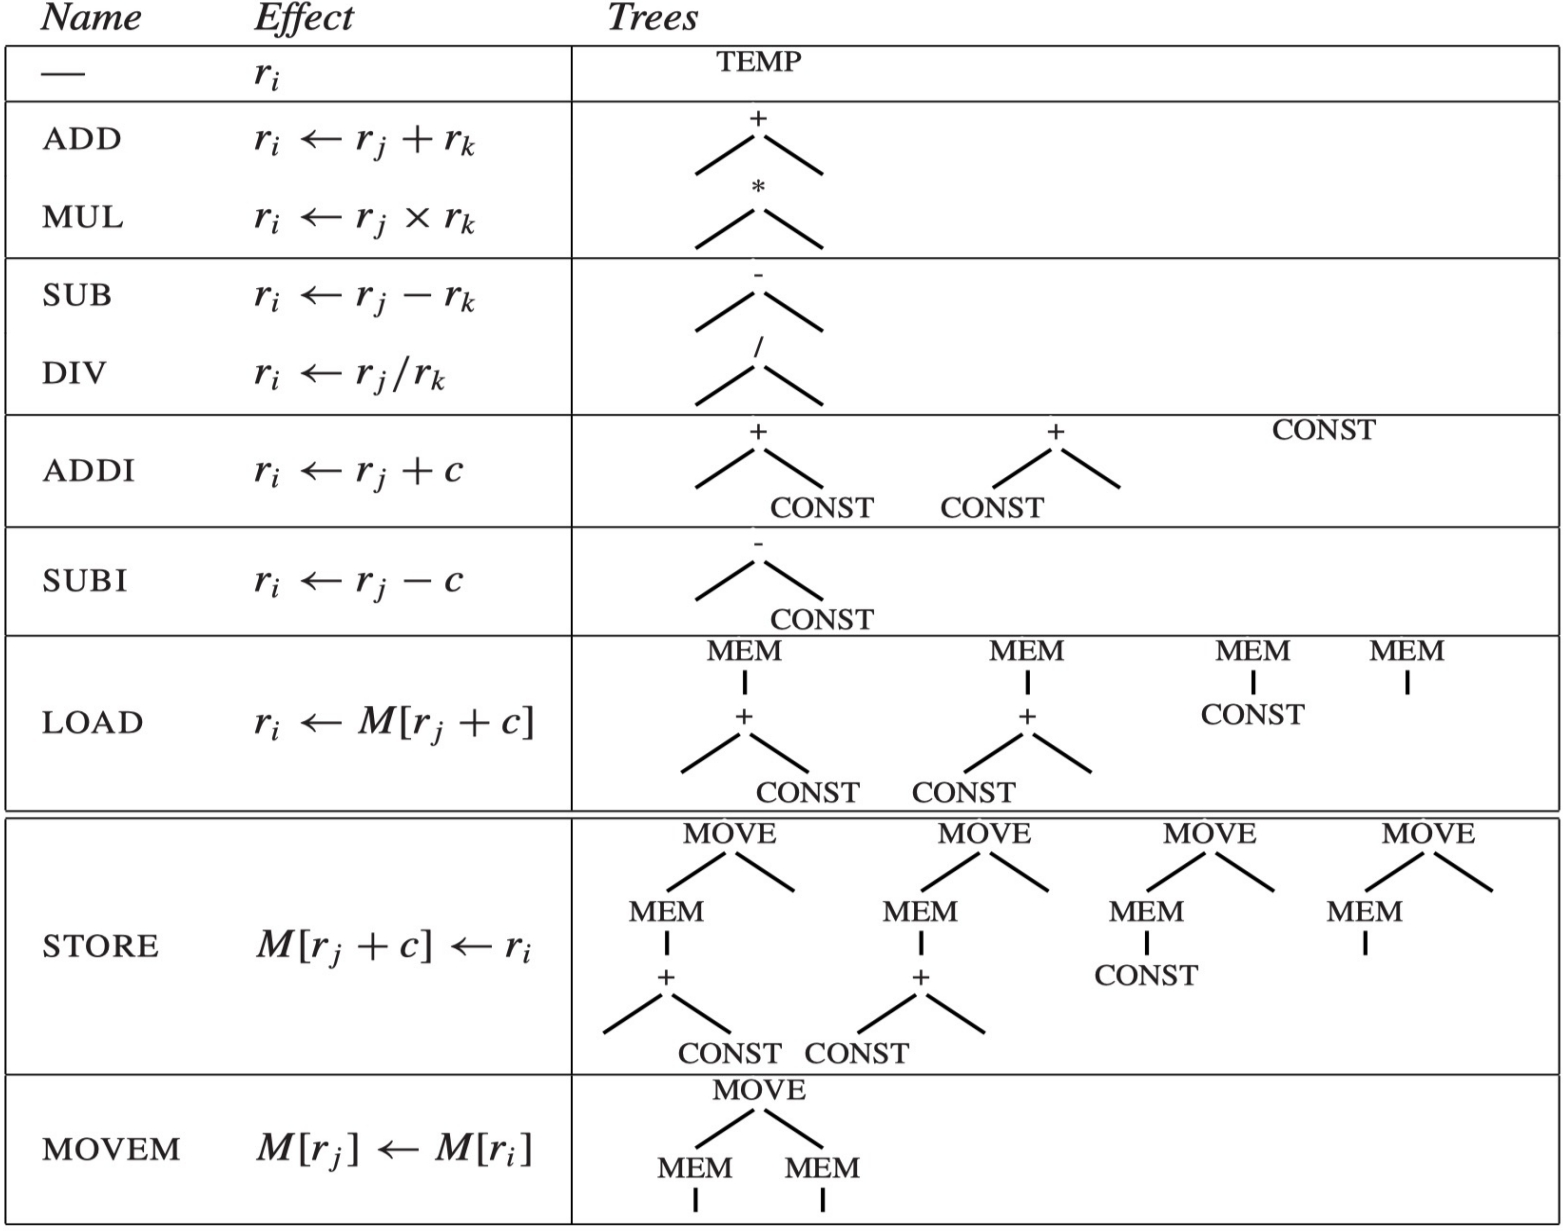
\includegraphics[width=\linewidth]{figures/is1.png}
\end{figure}

\par \noindent Optimum Tiling: 全局最优,整体代价最低;Optimal Tiling: 局部最优,每个片段最优但整体不一定最优。

\par \noindent Maximal Munch 算法:找到 Optimal Tiling。这是一个贪心算法,认为选择越大(节点数越多)的 Tile 导致的代价越小。
遇到相同大小的 Tile 任选其一。
从 IR 树的根节点开始,每次选择能够覆盖当前节点的最大图块,这将把原先的 IR 树分割为若干子树。
对每个被分割出的子树,重复相同的算法。
在完成 Tile 的放置后,以相反的顺序生成指令(从叶节点向根节点生成)。

\par \noindent 动态规划:找到 Optimum Tiling(一旦最小代价 tiling 的所有子树都被找到,那么根据这些子树的代价可以确定根节点的最小代价 tiling)。
自下而上地计算每个节点的最小成本。对于每个节点,首先计算其子节点的最小总成本 Tiling。每个节点的成本 := 所选 Tile 的成本 + 产生的子树的成本。
对于节点 $x$,定义 $f(x)$ 为以 $x$ 为根节点的树的 Optimal Tiling 的总成本,$f(x)$ 以下面的公式计算: 
\vspace{-10pt}
$$
f(x) = \min_{\forall T\text{ covering }x}\left( \text{cots}(T) + \sum_{\forall \text{ child }y\text{ of tile }T}f(y) \right)
$$
\vspace{-15pt}
\par \noindent 当整棵 IR 树的根节点的最小代价被找到,根据 IR 树的所有结点的代价状态,可以确定指令的选择(这个过程被称为 instruction emission),方法为:

\begin{figure}[H]
    \centering
    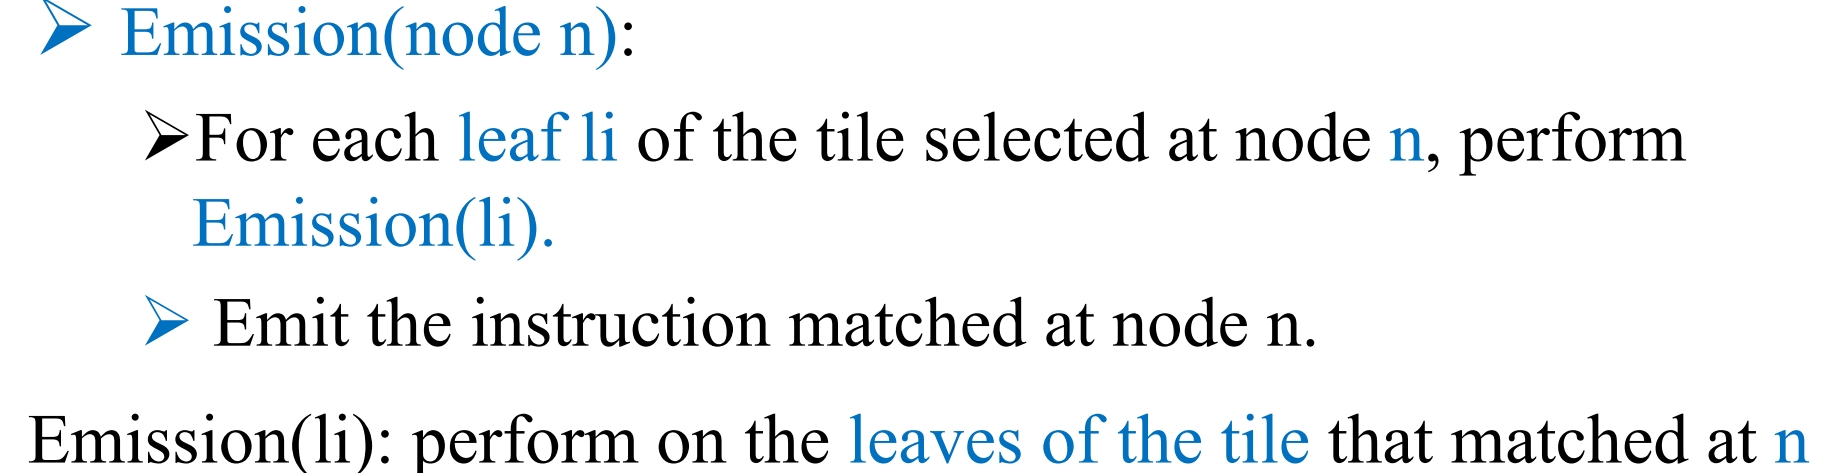
\includegraphics[width=0.8\linewidth]{figures/is2.png}
\end{figure}

\par \noindent Tree Grammar:对于 CISC 架构,对代码生成器中的 tile 进行硬编码可能很繁琐且 error-prune,
使用 Tree Grammar(一种特殊的 CFG)来描述图块,将指令选择简化为 parse 问题,使用动态规划算法进行 parse。
Tile 之间的关系被编码为重写规则,每个规则包括:Tree Grammar 中的产生式、Tile 的代价、翻译模板。
Tree Grammar 可能有二义性(有许多不同的指令序列实现相同的表达式),因此使用 DP。

% ======================================================
\par \noindent CISC 架构的其他问题【解决方案】:
1. 寄存器较少【不限制生成 TEMP 节点,假设寄存器分配能完成分配工作】;
2. 寄存器分类【将操作数显示地传送到相应的寄存器中】;
3. 两地址指令【增加一条额外的传送指令】;
4. 算数运算可以访问存储器【指令选择阶段将每一个 TEMP 节点转化成一个寄存器引用】;
5. 若干种寻址模式【这是优点,破坏寄存器少;指令代码短】;
6. 变长指令【不管】;
7. 副作用指令【三种解决办法:忽略地址自增指令、在采取树型匹配的代码生成器的上下文中使用特别方式匹配特殊的习惯用法、使用完全不同的指令算法,基于 DAG 样式】。
% ======================================================
% reference: https://github.com/Tian42chen/Transcription-Malfunctioned/blob/main/Compiler%20Principle/content/CP-CheatSheet9.tex
